% arara: lualatex: { synctex: on, shell: off }
% arara: biber
% arara: lualatex: { synctex: on, shell: off }
% arara: sumatrapdf
\documentclass[../main.tex]{subfiles}

% %Set the package to import preambles
\usepackage{subfiles}

%Load graphicx here to specify options
\usepackage[final]{graphicx}

%Set the document font
\usepackage[no-math]{fontspec}
\setmainfont[Ligatures=TeX]{Times New Roman}
\setmonofont{Inconsolata}

%Set the text to double spacing
%According to hyperref README,
%setspace should be loaded first
\usepackage[doublespacing]{setspace}

%Set a command to easily skip a line
\newcommand{\blankline}{\vspace*{\baselineskip}}

%Set up biblatex
\usepackage[
    backend=biber,
    % url=false,
    doi=true,
    sorting=none,
    sortcites=true,
    maxbibnames=6,
    minbibnames=6,
    maxcitenames=2,
    mincitenames=1,
    citestyle=numeric-comp,
    firstinits=true,
    isbn=false
]{biblatex}
\addbibresource{C:/Users/\user/Documents/Github/dissertation/library.bib}

%Remove the "In:" from before the journal title for articles
\renewbibmacro{in:}{%
  \ifentrytype{article}{}{\printtext{\bibstring{in}\intitlepunct}}}

%Change the name of the bibliography section to "References"
\DefineBibliographyStrings{english}{bibliography = {References}}

%Set the sort order of the names in each bibliography entry
\DeclareNameAlias{default}{last-first}

%Don't print the article title. To print the title, add #1 to the last {}
\DeclareFieldFormat[article,incollection,unpublished]{title}{}

%Add "vol." and "no." before volume and issue.
\DeclareFieldFormat[article]{volume}{\bibstring{volume}\addspace #1}
\DeclareFieldFormat[article]{number}{\bibstring{number}\addspace #1}

%Ensure that a comma follows abbreviated journal titles.
\DeclareFieldFormat{journaltitle}{\mkbibemph{#1}\isdot}

%Put a comma between the volume and issue instead of period.
\renewbibmacro*{volume+number+eid}{%
  \printfield{volume}%
  \setunit{\addcomma\space}%<---- was \setunit*{\adddot}%
  \printfield{number}%
  \setunit{\addcomma\space}%
  \printfield{eid}}

%Add a comma after the journal title.
\renewbibmacro*{journal+issuetitle}{%
  \usebibmacro{journal}%
  \setunit*{\addcomma\addspace}%<---- was \setunit*{\addspace}%
  \iffieldundef{series}
    {}
    {\newunit
     \printfield{series}%
     \setunit{\addspace}}%
  \usebibmacro{volume+number+eid}%
  \setunit{\addspace}%
  \usebibmacro{issue+date}%
  \setunit{\addcolon\space}%
  \usebibmacro{issue}%
  \newunit}

%Only print URL if doi is not present.
\DeclareFieldFormat{url}{%
  \iffieldundef{doi}{%
    \mkbibacro{URL}\addcolon\space\url{#1}%
  }{%
  }%
}
\DeclareFieldFormat{urldate}{%
  \iffieldundef{doi}{%
    \mkbibparens{\bibstring{urlseen}\space#1}%
  }{%
  }%
}

%Remove publisher from being printed.
\renewbibmacro*{publisher+location+date}{%
  \printlist{location}%
  \setunit*{\addcomma\space}%
  \usebibmacro{date}%
  \newunit}

%Fix in-text full citations
\DeclareCiteCommand{\fullcite}
  {\usebibmacro{prenote}}
  {\usedriver
     {\defcounter{minnames}{99}%
      \defcounter{maxnames}{99}}
     {\thefield{entrytype}}}
  {\multicitedelim}
  {\usebibmacro{postnote}}

%Use fancy tables.
\usepackage{booktabs}

%Set up todo notes in the PDF file
\usepackage{todonotes}

%Use and set up the caption package for nicer captions.
\usepackage{caption}
\DeclareCaptionLabelFormat{bf}{\textbf{#1 #2}}
\captionsetup{
    font=small ,
    labelsep=colon ,
    labelformat=bf ,
    figurewithin=chapter ,
    tablewithin=chapter ,
}

\usepackage{titlesec}
\usepackage{titletoc}

\titleformat{\chapter}[display]{\normalfont\Huge\bfseries}{Chapter \thechapter}{0.7em}{}
\titleformat{\section}{\normalfont\LARGE\bfseries}{\thesection}{0.5em}{}
\titleformat{\subsection}{\normalfont\Large\bfseries}{\thesubsection}{1em}{}
\titleformat{\subsubsection}{\normalfont\large\bfseries}{\thesubsubsection}{1em}{}

\titlecontents{chapter}[0pc]{}{\bfseries Chapter \thecontentslabel\quad}{}{\titlerule*[0.5pc]{.}\contentspage}
\titlecontents{section}[1em]{}{\thecontentslabel\quad}{}{\titlerule*[0.5pc]{.}\contentspage}
\titlecontents{subsection}[2em]{}{\thecontentslabel\quad}{}{\titlerule*[0.5pc]{.}\contentspage}
\titlecontents{subsubsection}[3em]{}{\thecontentslabel\quad}{}{\titlerule*[0.5pc]{.}\contentspage}

\setcounter{secnumdepth}{3}
\setcounter{tocdepth}{3}

%Use the subfigure package
\usepackage{subfig}

%Various math improvements.
%Must be loaded before hyperref
\usepackage{mathtools}

%Set the math font. Has to come after mathtools because
%some font stuff gets overwritten.
\usepackage{unicode-math}
\unimathsetup{math-style=TeX}
\setmathfont[range=\mathup/{num}]{Times New Roman}
\setmathfont[range=\mathit/{greek,Greek,latin,Latin}]{Cambria Math}
\setmathfont[range=\mathup/{greek,Greek,latin,Latin}]{Cambria Math}
\setmathfont[range={"2212,"002B,"003D,"0028,"0029,"005B,"005D,"221A,
"2211,"2248,"222B,"007C,"2026,"2202,"00D7,"0302,"2261,"0025,"22C5,
"00B1,"2194,"21D4,"2260}]
{Cambria Math}

%Better looking fonts
\usepackage[final]{microtype}

%Allow table cells to span multiple rows.
\usepackage{multirow}

%Allow landscape rotated figures and captions.
\usepackage{afterpage}
\usepackage{rotating}
\usepackage{pdflscape}

%Set the root path where figures are stored.
\graphicspath{ {C:/Users/\user/Documents/Github/dissertation/figures/} }

%Set a convenience command for table cells that allow line breaks.
\newcommand{\linebreakcell}[2][c]{%
  \begin{tabular}[#1]{@{}c@{}}#2\end{tabular}}

%Use and set up the siunitx package for nice units printing.
\usepackage{siunitx}
\sisetup{%
    group-separator = {,},
    range-phrase = {\text{ to }},
    list-separator = {\text{, }},
    list-final-separator = {\text{, and }},
    list-pair-separator = {\text{ and }},
}%
\DeclareSIUnit\calorie{cal}
\DeclareSIUnit\atmosphere{atm}
\DeclareSIUnit\torr{torr}

%Declare convenience macros for printing the
%names of the alcohols.
\newcommand{\iPeOH}{\textit{i}-pentanol}
\newcommand{\nBuOH}{\textit{n}-butanol}
\newcommand{\sBuOH}{\textit{s}-butanol}
\newcommand{\tBuOH}{\textit{t}-butanol}
\newcommand{\iBuOH}{\textit{i}-butanol}

%The floatrow package allows multiple floats in a row
%and is set so that table captions are on top of the
%table.
\usepackage{floatrow}
\floatsetup[table]{style=plaintop}

%Use the titling package to allow easy access to custom title pages
\usepackage{titling}
\title{High Pressure Ignition Chemistry of Alternative Fuels}
\author{Bryan William Weber}

%Add bibliography and indices to the TOC
\usepackage{tocbibind}

%Improve handling of appendices
\usepackage{appendix}

%Use package that allows inline patching of commands. This is used in
%the appendices section.
\usepackage{xpatch}

%Use the bookmark package (which loads hyperref) so that only one
%compilation is necessary to get references.
\usepackage{bookmark}

%Set the color of the links and PDF metadata
\hypersetup{%
    pdfinfo={
        Title={High Pressure Ignition Chemistry of Alternative Fuels},
        Author={Bryan W. Weber},
    },
    colorlinks=true,
    citecolor=blue,
    linkcolor=black,
    plainpages=false,
    final,
}

%Allow lualatex to properly add links processed from pax files.
\usepackage{pdftexcmds}
\makeatletter
\let\pdfescapename=\pdf@escapename
\let\pdfstrcmp=\pdf@strcmp
\makeatother
\usepackage{pax}

%Allow to use \doi to link to DOI links.
\usepackage{doi}

%Allow inserting PDF documents directly to the output. According to
%http://tex.stackexchange.com/a/13660/32374, should come after hyperref
\usepackage{pdfpages}

%Do a better job with the automatic references. According to
%http://tex.stackexchange.com/a/1868/32374, should come after hyperref
\usepackage[capitalise, sort&compress]{cleveref}

%Set the auto-format names for the cleveref operations
\crefname{chapter}{Chapter}{Chapters}
\Crefname{chapter}{Chapter}{Chapters}
\crefname{section}{Sec.}{Secs.}
\Crefname{section}{Section}{Sections}
\crefname{subsection}{Sec.}{Secs.}
\Crefname{subsection}{Section}{Sections}
\crefname{subsubsection}{Sec.}{Secs.}
\Crefname{subsubsection}{Section}{Sections}
\crefname{figure}{Fig.}{Figs.}
\Crefname{figure}{Figure}{Figures}
\crefname{table}{Table}{Tables}
\Crefname{table}{Table}{Tables}
\crefname{equation}{Eq.}{Eqs.}
\Crefname{equation}{Equation}{Equations}
\crefname{appchap}{Appendix}{Appendices}
\Crefname{appchap}{Appendix}{Appendices}

\newcommand{\creflastconjunction}{, and~}
\newcommand{\crefrangeconjunction}{--}

%Set the size of the margins and the paper
%According to http://tex.stackexchange.com/a/26592/32374
%this should go after hyperref
\usepackage[margin=1in, letterpaper]{geometry}

%Set up the page numbers
%This has to go after geometry so the page number is centered
\usepackage{fancyhdr}
\pagestyle{fancy}
\fancyhf{}
\fancyfoot[C]{\thepage}
\renewcommand{\headrulewidth}{0pt}


\begin{document}

\begin{figure}[!ht]\CenterFloatBoxes
    \begin{floatrow}
        \killfloatstyle\ttabbox[10cm]
            {\captionsetup{type=table}\caption{Molar Proportions of Reactants in MCH Experiments}
            \label{tab:mch-props}}
            {\begin{tabular}{*{6}{S}}
            \toprule
            {Mix \#} & {$\phi$} & {MCH} & {O$_2$} & {N$_2$} & {Ar} \\
            \midrule
            1 & 1.0 & 1 & 10.5 & 12.25 & 71.75 \\
            2 & 0.5 & 1 & 21.0 &  0.00 & 73.50 \\
            3 & 1.5 & 1 &  7.0 & 16.35 & 71.15 \\
            \bottomrule
            \end{tabular}
            }
        \ffigbox[5cm]
            {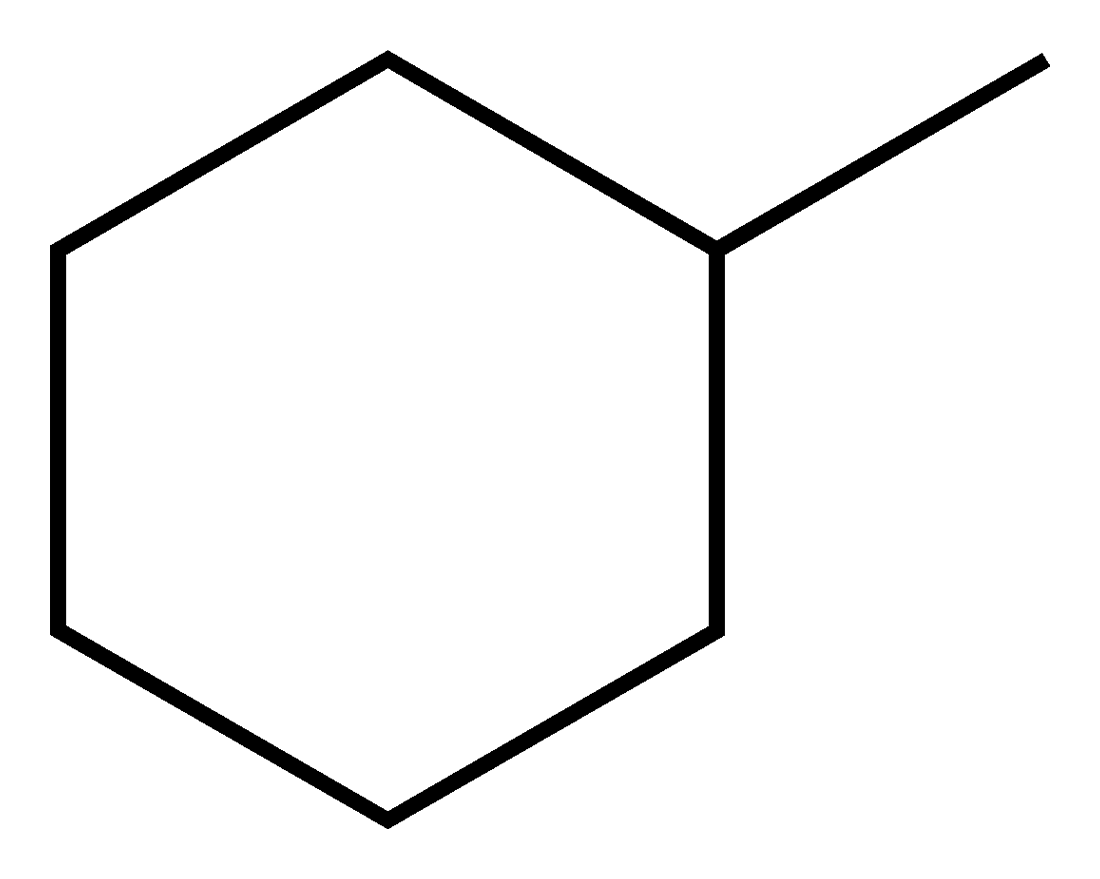
\includegraphics[width=3cm]{05-MCH/mch-skeletal}}
            {\caption{Skeletal structure of methylcyclohexane}
            \label{fig:mch-skeletal}}
    \end{floatrow}
\end{figure}

\section{Structure of Methylcyclohexane}
\label{sec:mch-structure}

Methylcyclohexane (MCH) is the simplest branched cycloalkane, and as such,
represents an excellent target to use as the base for models of larger
branched cycloalkanes. MCH has the elemental composition C$_7$H$_{14}$, and
its skeletal structure is shown in \cref{fig:mch-skeletal}.

\section{Procedures}
\label{sec:mch}

The liquid fuel (methylcyclohexane, \SI{99.0}{\percent} purity) is massed to a precision
of \SI{0.01}{\gram} in a syringe before being injected into the mixing tank through a
septum. The proportions of oxygen (\SI{99.9999}{\percent} purity), nitrogen (\SI{99.9995}{\percent}
purity), and argon (\SI{99.9999}{\percent} purity) are determined by specifying the oxidizer
composition, the equivalence ratio, and the total mass of fuel. The gases are
added to the mixing tank manometrically at room temperature.

Three different mixtures of MCH/O$_2$/N$_2$/Ar are prepared in this study, as
outlined in \cref{tab:mch-props}. These mixtures (denoted as Mix \#1--3) match the mixtures
prepared in our previous work with MCH in the RCM \cite{Mittal2009}. The equivalence ratios
corresponding to Mix \#1--3 are $\phi=\numlist{1.0;0.5;1.5}$, respectively.
As in the previous RCM experiments, the mole fraction of MCH is held constant
and the mole fraction of O$_2$ is varied to adjust the equivalence ratio. This
experimental design allows these data to be used to validate chemical kinetic
models for changes in O$_2$ concentration, which is an important variable in
internal combustion engines where exhaust gas recirculation is used to reduce
the oxygen concentrations to avoid NOx formation. Few validation data for
ignition are available for changing oxygen concentrations. In addition, the
relative proportions of O$_2$, N$_2$, and Ar are adjusted so that the same specific
heat ratio is maintained in the three mixtures. As discussed in \cref{sec:reac-temp},
$P_C$ and $T_C$ are assumed to only depend on the temperature-dependent
specific heat ratio of the reactants, the compression ratio, and the
initial conditions. Thus, for given $P_C$, compression ratio, and
initial conditions, the $T_C$ will be similar for all the equivalence
ratios in these experiments.

\section{Model Improvements}
\label{sec:mch-model-improvements}

Through collaboration with researchers at Lawrence Livermore National
Laboratory (LLNL), many improvements to the chemical kinetic model for MCH were
made. Some of the major improvements are highlighted below; see the article
for more detail \cite{Weber2014}. It should be noted that the improvement relative to the model
from 2007 by \textcite{Pitz2007} is substantial.

\begin{enumerate}
    \item The base C$_1$--C$_4$ chemistry has been updated with the AramcoMech
        version 1.3 \cite{Metcalfe2013}.
    \item The aromatics base chemistry was updated with the latest LLNL-NUIG
        model \cite{Nakamura2014}.
    \item The cyclohexane sub-model was updated with a new version from
        \textcite{Silke2007}.
    \item Rates of abstraction reactions from MCH have been updated
        with recently measured experimental values \cite{Sivaramakrishnan2009}
        and standardized according to the LLNL reaction rate rules \cite{Sarathy2011b}.
    \item Products of MCH breakdown with unsaturated rings such as
        methylcyclohexene were previously lumped into one species for
        simplicity. In the new model, they have been unlumped and
        provide improved fidelity in modeling these species. \cite{Pitz2013}.
    \item The reaction rates of some low-temperature specific reactions were
        updated using new quantum chemical calculations to compute the rate.
        Other reaction rates were updated from similar calculations performed
        by \textcite{Fernandes2009}.
    \item The activation energy of the ketohydroperoxide decomposition
        reactions was increased to bring it into closer agreement with
        the activation energy used by \textcite{Metcalfe2013}. This change
        has a dramatic effect on the low-temperature ignition delays, as shown
        in \cref{sec:model-comparison}.
\end{enumerate}

\section{Experimental Results}
\label{sec:mch-expts}

The experimental ignition delays measured at the three equivalence ratios and
compressed pressure of \SI{50}{\bar} are shown in \cref{fig:mch-expts}. The open symbols are the
overall ignition delays, and the filled symbols are the first stage ignition
delays. The vertical error bars on the experimental data represent twice the
standard deviation of all of the experiments at that condition as
discussed in \cref{sec:ign-delay-def}. Detailed uncertainty analysis of
the deduced compressed temperature was conducted as reported in
\cref{sec:unc-mch} where the uncertainty of the compressed
temperature was estimated to be approximately \SI{1}{\percent}.

\begin{figure}
    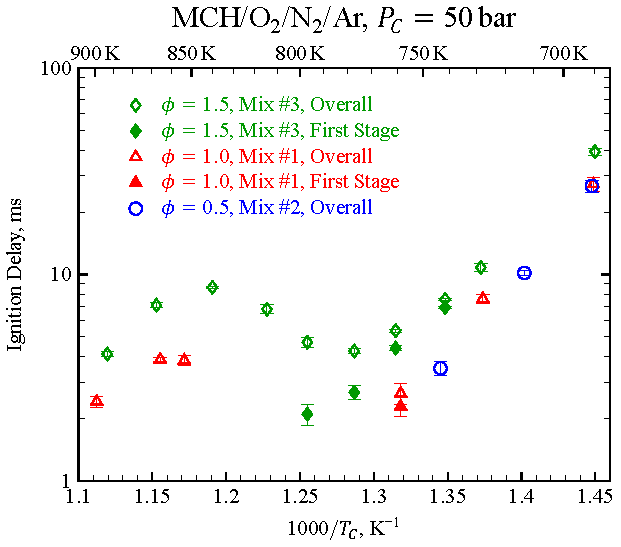
\includegraphics[width=9cm]{05-MCH/mch-expts}
    \caption{Experimentally measured ignition delays at $P_C=\SI{50}{\bar}$ for the
    mixture conditions in \cref{tab:mch-props}}
    \label{fig:mch-expts}
\end{figure}

The negative temperature coefficient (NTC) region is an important feature of
low temperature ignition where the ignition delay time increases with
increasing temperature. The NTC region of the overall ignition delay is
evident in \cref{fig:mch-expts} for the $\phi=\num{1.5}$ case (Mix \#3) and
approximately includes the temperature range of $T_C=\SIrange{775}{840}{\kelvin}$. For
$\phi=\num{1.5}$, first stage ignition is evident for conditions in the range of
$T_C=\SIrange{740}{800}{\kelvin}$.

For $\phi=\num{1.0}$ (Mix \#1), the NTC region of the overall ignition delay could
not be completely resolved. Only three conditions in the low temperature region
and three conditions in the high temperature region are shown in
\cref{fig:mch-expts}. The experimental pressure traces during the compression
stroke for intermediate temperature conditions deviated from their
non-reactive counterparts, demonstrating appreciable reactivity therein. Hence,
those data are not included in \cref{fig:mch-expts}.

For the experiments at $\phi=\num{0.5}$ (Mix \#2), only three data points in the low
temperature region are reported and none of them exhibit two-stage ignition
response. As the temperature is increased further, noticeable reactivity during
the compression stroke is evident.

As stated earlier, the mole fraction of MCH is held constant in this study,
while the mole fraction of the oxidizer is changed to modify the equivalence
ratio. \Cref{fig:mch-expts} demonstrates that the $\phi=\num{0.5}$ case is the most
reactive (as judged by the inverse of the ignition delay) and the $\phi=\num{1.5}$
case is the least reactive. As has been shown for other fuels, including
\textit{n}-butanol \cite{Weber2011} and Jet-A \cite{Kumar2010}, decreasing the
equivalence ratio by increasing the oxygen mole fraction but holding the fuel
mole fraction constant increases the reactivity.

\section{Comparison to Model}
\label{sec:model-comparison}

A comparison of the experimentally measured first stage ignition delays (open
symbols) and the first stage ignition delays computed using the updated model
(lines) is shown in \cref{fig:mch-model-1-first,fig:mch-model-2-first,,%Comma necessary to avoid compression
fig:mch-model-3-first} for Mix \#1, \#2, and \#3. In
addition, a comparison of the experimentally measured overall ignition delays
(open symbols) and the overall ignition delay computed by the updated model
(lines) is shown in \cref{fig:mch-model-1-over,fig:mch-model-2-over,,%
fig:mch-model-3-over}. The experiments include the new work being
presented here at $P_C=\SI{50}{\bar}$ in addition to the previous RCM experiments at
$P_C=\SIlist{15.1;25.5}{\bar}$ \cite{Mittal2009}. The simulations are of
the VPRO type. For some computational cases, substantial heat release during
the compression stroke caused the computed pressure to depart from the
non-reactive profile prior to EOC. Therefore, these cases are not shown in
\cref{fig:mch-model-1,fig:mch-model-2,fig:mch-model-3}. For these conditions, the
experimental pressure trace did not exhibit significant heat release during
the compression stroke and the experimental pressure at EOC for the reactive
case matched that of the non-reactive counterpart.

\begin{figure}
    \floatsetup[subfigure]{captionskip=6pt}
    \ffigbox{%
        \begin{subfloatrow}
            \ffigbox
                {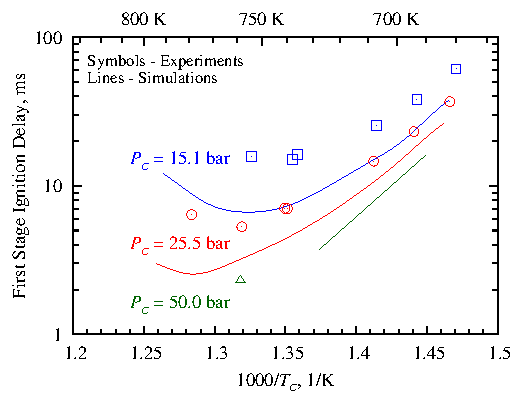
\includegraphics[width=7cm]{05-MCH/mch-model-1-first}}
                {\caption{First stage ignition delays}\label{fig:mch-model-1-first}}
            \ffigbox
                {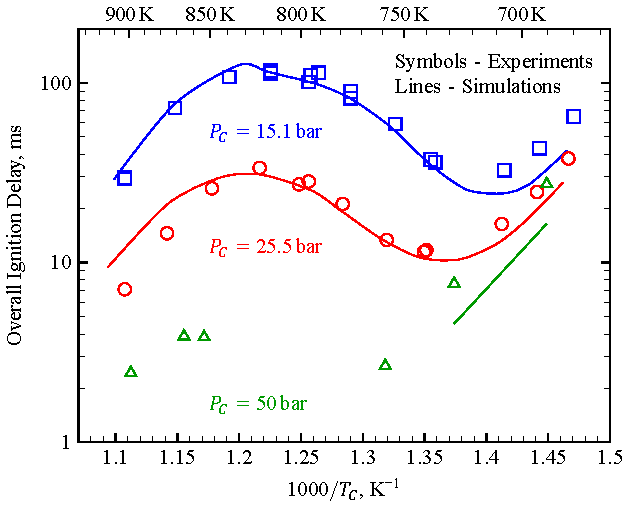
\includegraphics[width=7cm]{05-MCH/mch-model-1-over}}
                {\caption{Overall ignition delays}\label{fig:mch-model-1-over}}
        \end{subfloatrow}
    }%
    {\caption{Comparison of experimental and simulated ignition delays for three
        pressures for Mix \#1. The data at \SIlist{15.1;25.5}{\bar} are from the
        study of \textcite{Mittal2009}.}
        \label{fig:mch-model-1}}
% \end{figure}
\par
\vspace{7pt}
% \begin{figure}
    \ffigbox{%
        \begin{subfloatrow}
            \ffigbox
                {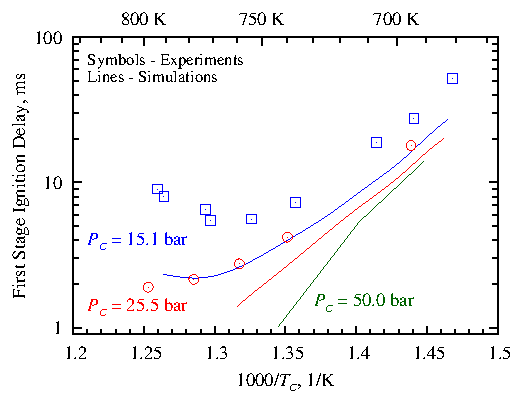
\includegraphics[width=7cm]{05-MCH/mch-model-2-first}}
                {\caption{First stage ignition delay}\label{fig:mch-model-2-first}}
            \ffigbox
                {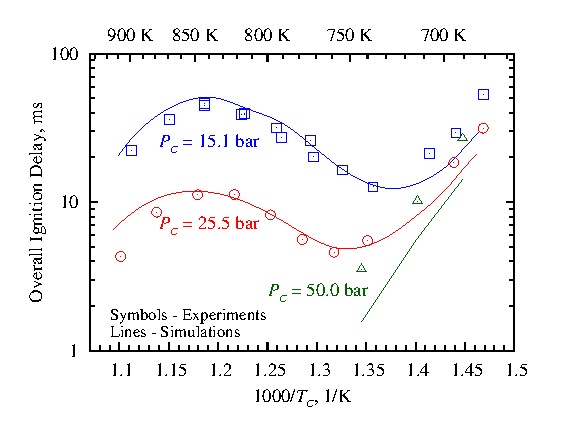
\includegraphics[width=7cm]{05-MCH/mch-model-2-over}}
                {\caption{Overall ignition delay}\label{fig:mch-model-2-over}}
        \end{subfloatrow}
    }%
    {\caption{Comparison of experimental and simulated ignition delays for three
        pressures for Mix \#2. The data at \SIlist{15.1;25.5}{\bar} are from the
        study of \textcite{Mittal2009}.}
    \label{fig:mch-model-2}}
% \end{figure}
\par
\vspace{7pt}
% \begin{figure}
    \ffigbox{%
        \begin{subfloatrow}
            \ffigbox
                {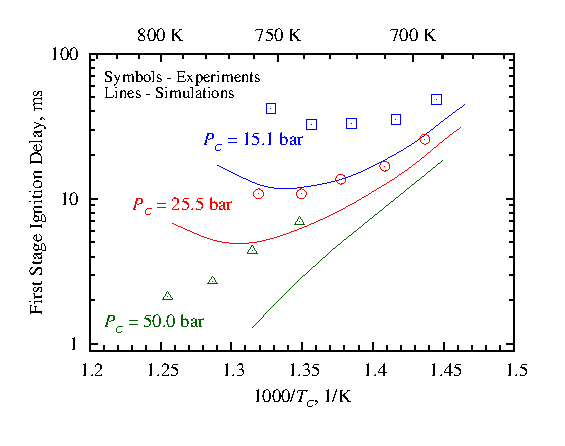
\includegraphics[width=7cm]{05-MCH/mch-model-3-first}}
                {\caption{First stage ignition delay}\label{fig:mch-model-3-first}}
            \ffigbox
                {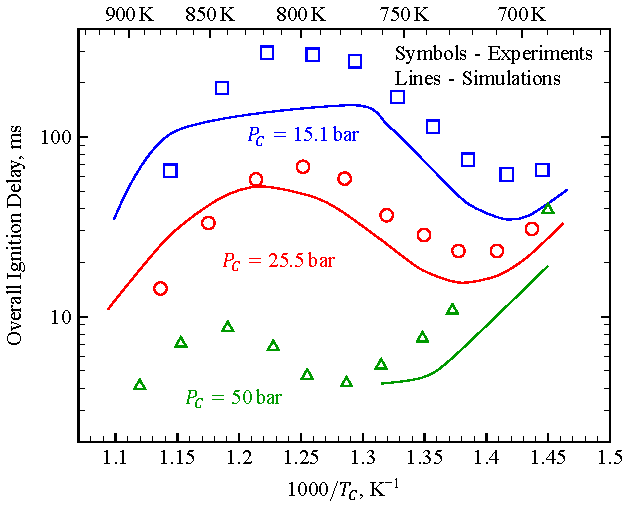
\includegraphics[width=7cm]{05-MCH/mch-model-3-over}}
                {\caption{Overall ignition delay}\label{fig:mch-model-3-over}}
        \end{subfloatrow}
    }%
    {\caption{Comparison of experimental and simulated ignition delays for three
        pressures for Mix \#3. The data at \SIlist{15.1;25.5}{\bar} are from the
        study of \textcite{Mittal2009}.}
    \label{fig:mch-model-3}}
\end{figure}

At \SIlist{15.1;25.5}{\bar} for Mix \#1 and \#2, the overall ignition delay is very
well predicted for temperatures above approximately \SI{715}{\kelvin}. For lower
temperatures at these two equivalence ratios, the experimental ignition delays
are under-predicted by the model, but the predictions are nevertheless within
a factor of two of the data. For the rich case (Mix \#3), the simulations
under-predict the ignition delay over a wider temperature range but the results
improve as temperature increases. Again, the experimental ignition delays are
predicted to within approximately a factor of two. At \SI{50}{\bar}, the ignition
delays are under-predicted for all of the equivalence ratios studied here, but
the agreement is within a factor of two.

The first stage ignition delays for all of the pressure and equivalence ratios
are under-predicted, but are within a factor of three of the experimental
values. Furthermore, for all of the equivalence ratios tested at $P_C=\SI{50}{\bar}$,
it is of interest to note that there are several cases where simulated ignition
delays show two-stage response where the experiment shows only a single stage
ignition. Nevertheless, the present mechanism is a marked improvement from the
comparison performed by \textcite{Mittal2009} who found that the ignition
delays were strongly and uniformly over-predicted by the previous LLNL
mechanism by \textcite{Pitz2007}.

\Cref{fig:mch-pressure} shows a comparison of selected simulated and
experimentally measured pressure traces for Mix \#1, \#2, and \#3 at
$P_C=\SI{50}{\bar}$. Also shown in \cref{fig:mch-pressure} is the
simulated non-reactive pressure trace corresponding to each experimental
condition. Small differences in the heat loss profile for different
temperatures are apparent in the non-reactive pressure traces. These
differences arise from the changing surface area to volume ratio of the
reaction chamber at the end of compression as the compression ratio is changed
to vary the compressed temperature. This highlights the importance of using
VPRO simulations to compare predictions of ignition delay with the experimental data.

For Mix \#1, it is clear that the simulated reactive pressure trace in
\cref{fig:mch-pressure-1} at $T_C=\SI{866}{\kelvin}$ (red dashed line) deviates from
the non-reactive pressure trace (red dot-dot-dashed line) prior to the end of
compression. The same is also true of the \SI{797}{\kelvin} case shown for Mix \#3 in
\cref{fig:mch-pressure-3}. Remarkably, the simulated case for Mix \#1 at
$T_C=\SI{866}{\kelvin}$ (\cref{fig:mch-pressure-1}, red dashed line)
predicts the overall ignition delay quite well. However, due to the
heat release prior to EOC, this simulated result is not plotted in
\cref{fig:mch-model-1}. The simulated case for Mix \#3 at $T_C=\SI{797}{\kelvin}$ is also
not plotted on \cref{fig:mch-model-3} due to the heat release prior to EOC;
interestingly, this case under-predicts the first stage ignition delay but
over-predicts the overall ignition delay. For the other simulated cases (black
lines), the reactive pressure traces closely follow their non-reactive
counterparts until the ignition event begins. The experimental ignition delays
of these cases are under-predicted by the model. It is also seen in
\cref{fig:mch-pressure-3} for $T_C=\SI{729}{\kelvin}$ that the model predicts two-stage
ignition, although two-stage ignition is not observed experimentally.

\begin{figure}
    \floatsetup[subfigure]{floatrowsep=none}
    \ffigbox{%
        \begin{subfloatrow}[3]
            \ffigbox
                {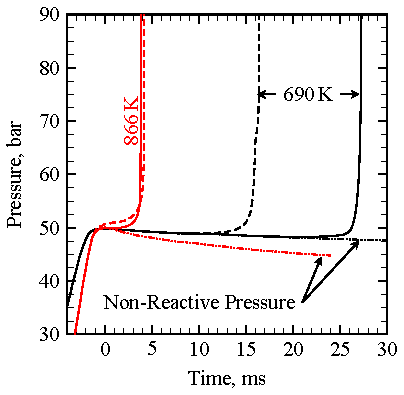
\includegraphics[height=5.35cm]{05-MCH/mch-pressure-1}}
                {\caption{Mix \#1}\label{fig:mch-pressure-1}}
            \ffigbox
                {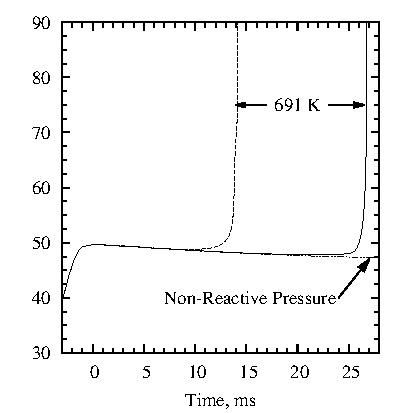
\includegraphics[height=5.35cm]{05-MCH/mch-pressure-2}}
                {\caption{Mix \#2}\label{fig:mch-pressure-2}}
            \ffigbox
                {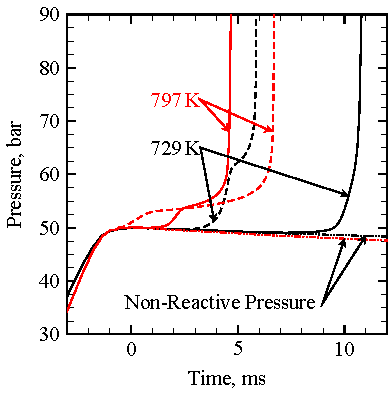
\includegraphics[height=5.35cm]{05-MCH/mch-pressure-3}}
                {\caption{Mix \#3}\label{fig:mch-pressure-3}}
        \end{subfloatrow}
    }
    {\caption{Comparison of selected simulated and experimental pressure traces
        at $P_C=\SI{50}{\bar}$. Red lines
        indicate that the pressure profile of the reactive simulation deviates
        from the non-reactive case prior to EOC. Solid lines: experiment;
        dashed lines: reactive simulation; dot-dot-dashed lines: non-reactive
        simulation.}
    \label{fig:mch-pressure}}
\end{figure}

The current mechanism is also compared to shock tube ignition delays from the
studies of \textcite{Vasu2009} and \textcite{Vanderover2009}. Those studies
considered the autoignition of stoichiometric mixtures of MCH with O$_2$/N$_2$
air. The comparison is shown in \cref{fig:mch-shocks} for the near \SI{50}{atm}
data from those studies. Note that the experimental data shown are the raw
data and are not scaled to a constant pressure, whereas the simulated
ignition delays are at a constant initial pressure of \SI{50}{atm}. It can be seen
that the ignition delays are over-predicted over nearly the entire temperature
range of \SIrange{795}{1160}{\kelvin} studied. Nevertheless, the predicted ignition delays are
within approximately a factor of 1.5 of the experiments, indicating good
agreement overall and a substantial improvement from the previous version of
the model. Furthermore, the simulations shown here are of the CONV type and
do not account for any facility dependent effects present in the experiments.
Although the experimentalists noted in their studies \cite{Vasu2009,Vanderover2009} 
that the effect of such considerations is minimal, including facility
dependent effects will tend to make the simulations ignite sooner and improve
the agreement, especially for cases with ignition delays longer than
approximately \SI{1000}{\micro\second}.

As discussed in \cref{sec:mch-model-improvements}, one of the updates to the model
was to increase the activation energy of ketohydroperoxide decomposition, from
$E_a=\SI{39}{\kilo\calorie\per\mole}$ (\SI{163.2}{\kilo\joule\per\mole}) to
\SI{41.6}{\kilo\calorie\per\mole} (\SI{174.1}{\kilo\joule\per\mole}). This
update substantially improved the prediction of the low-temperature ignition
delays, including the first stage and overall ignition delays. As mentioned by
\textcite{Curran2002}, ``the high activation energy [of ketohydroperoxide
decomposition] ensures an induction period during which the ketohydroperoxide
concentration builds up.'' Furthermore, updating this activation energy does not
affect the high-temperature ignition delays. A comparison of calculated
ignition delays demonstrating the effect of this update is shown in
\cref{fig:mch-energy}.

\begin{figure}
    \begin{floatrow}
        \ffigbox
            {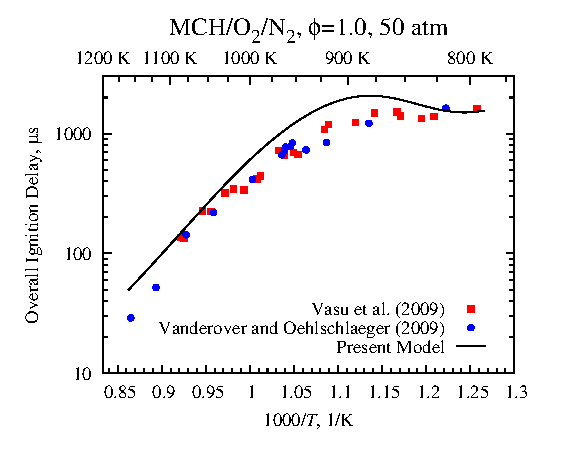
\includegraphics[width=7.9cm]{05-MCH/mch-shocks}}
            {\caption{Comparison of the present model with the experiments from
                \textcite{Vasu2009} and \textcite{Vanderover2009} near \SI{50}{atm}
                and for stoichiometric mixtures in O$_2$/N$_2$ air.}
            \label{fig:mch-shocks}}
        \ffigbox
            {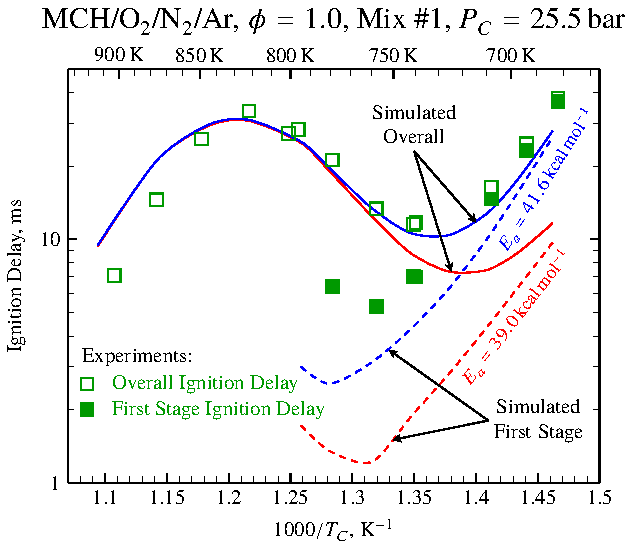
\includegraphics[width=7.9cm]{05-MCH/mch-energy}}
            {\caption{Comparison of mechanism performance with the activation energy
                of ketohydroperoxide decomposition set at \SI{41.6}{\kilo\calorie\per\mole} (blue) and
                \SI{39.0}{\kilo\calorie\per\mole} (red). Experimental ignition delays are shown in
                green symbols.}
            \label{fig:mch-energy}}
    \end{floatrow}
\end{figure}

\section{Discussion}
\label{sec:discussion}
\subsection{Path Analysis}
\label{sec:mch-path-analysis}

The relatively good agreement of the updated model with the experimental data
suggests that a more detailed analysis of the mechanism is a worthwhile
exercise and such analysis may point the way to further improvements to the
mechanism. We begin with a reaction path analysis. The present reaction path
analysis is conducted using a CONV (adiabatic, constant-volume) type simulation
for three initial temperatures (\SIlist{700;800;900}{\kelvin}), at \SI{25.5}{\bar} and for
Mix \#1 (the stoichiometric case). For the other mixture conditions and
pressures considered in this work, the absolute percentages for each channel
change slightly. However, the analysis of the reaction pathways is the same for
all of the equivalence ratios and pressures considered in the experiments
presented previously. The three temperatures considered in this analysis
correspond to the low-temperature, peak of the NTC, and high-temperature
portions of the ignition delay curve illustrated in \cref{fig:mch-energy};
their results are shown in \cref{fig:mch-path} with plain text, bold text,
and italic text, respectively.

The path analysis presented in \cref{fig:mch-path} is an integrated analysis
where the rate of production (ROP) of each species by each reaction has been
integrated with respect to time up to \SI{20}{\percent} fuel consumption. The integrated
ROPs from each reaction are normalized by the total production or destruction
of that species up to \SI{20}{\percent} fuel decomposition, such that reactions that produce
a species are normalized by the total production of the species and reactions
that consume a species are normalized by the total consumption of that species.
The percentages in \cref{fig:mch-path} therefore represent the percent of the given
reactant that is consumed to form the given product by all reactions that can
form a particular product. Species such as hydroperoxyalkyl radicals (QOOH),
alkyl hydroperoxides (ROOH), and methylcyclohexenes (MCH-ene) are shown as
lumped on the path diagram; however, these species are unlumped in the
mechanism and presented as a lumped sum for simplicity in this diagram. Note
that not all of the pathways present in the mechanism for each species are
presented in \cref{fig:mch-path}, again for simplicity; the pathways that are shown in
\cref{fig:mch-path} typically account for more than \SI{95}{\percent} of the consumption
of each species.

\begin{figure}
    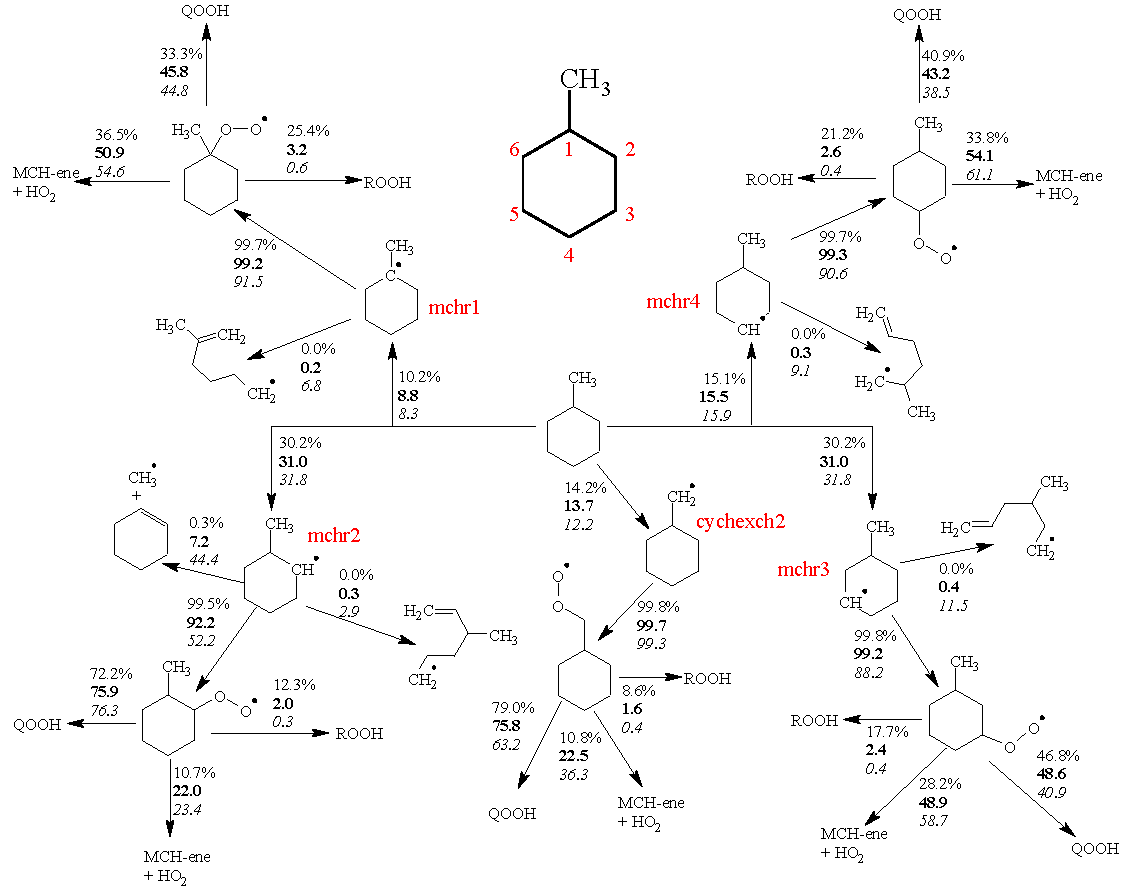
\includegraphics[width=\textwidth]{05-MCH/mch-path}
    \caption{Path analysis of MCH combustion. Initial conditions are 25.5 bar
    and Mix \#1 ($\phi=\num{1.0}$) and \SI{700}{\kelvin} (plain text),
    \SI{800}{\kelvin} (bold text), \SI{900}{\kelvin} (italic text).
    Note that not all possible reaction pathways are shown for
    each species.}
    \label{fig:mch-path}
\end{figure}

The first step of fuel breakdown occurs by H-atom abstraction at these pressure
and temperature conditions. None of the fuel is directly decomposed by
unimolecular reactions. Each of the seven possible radicals are formed in
comparable quantities; however, due to the symmetry of MCH, sites 2 and 3 are
equivalent to sites 6 and 5, respectively, so mchr2 and mchr3 have close to
double the production rate compared to the other radicals. It is interesting to
note that the production of mchr2, mchr3, and mchr4 increase as the initial
temperature increases and the production of mchr1 and cychexch2 decrease to
compensate. However, the change is small, no more than 2 percentage points for
each radical.

The most important second step is oxygen addition (i.e. formation of ROO) at
all of the initial temperatures in this analysis. The importance of this
reaction diminishes for each radical as the initial temperature increases due
to the increasing importance of $\beta$-scission reactions. At \SI{700}{\kelvin}, less than
\SI{0.05}{\percent} of each of the fuel radicals is consumed via $\beta$-scission. Between
\SIlist{800;900}{\kelvin}, the percentages of mchr1, mchr2, mchr3, and mchr4 that are decomposed
via $\beta$-scission increase by several thousand percent each; nevertheless,
the absolute change is small and the consumption of these radicals still occurs
mostly by oxygen addition. The mchr1, mchr3, and mchr4 radicals undergo
scission of the cyclohexyl ring, whereas mchr2 primarily undergoes scission at the
methyl-cyclohexyl bond. This beta scission of mchr2 competes significantly with
its consumption by O$_2$ at \SI{900}{\kelvin}. Furthermore, the increasing importance of the
ring opening reactions from \SI{800}{\kelvin} to \SI{900}{\kelvin} means that chain propagation pathways
(instead of effective chain termination pathways forming methylcyclohexene and
hydroperoxyl) are available, increasing the reactivity. Finally, even at the
elevated initial temperature of \SI{900}{\kelvin}, cychexch2 does not undergo significant
ring opening. Instead, it will scission an H atom from site 1 or steal an oxygen
atom from hydroperoxyl to form an alkoxy radical (RO) when it does not undergo
oxygen addition (these pathways each only consume about \SI{0.3}{\percent} of cychexch2 and
hence are not shown in \cref{fig:mch-path}).

Returning to the low temperature pathways, there are four important classes of
reactions that consume the ROO radicals in the current mechanism. These classes
are: C1) internal H-atom transfer (isomerization) to form QOOH; C2) direct
elimination of hydroperoxyl and methylcyclohexene; C3) H-abstraction by ROO
from either the fuel or hydroperoxyl to form ROOH; and, C4) reactions among the
ROO radicals. Class C4 consumes less than $\approx\SI{5}{\percent}$ of each of the ROO radicals at
\SI{700}{\kelvin} and less than $\approx\SI{0.1}{\percent}$ for the other temperatures and this class is
therefore not shown on the path diagram in \cref{fig:mch-path}. Of the other
three classes, C1 (formation of QOOH) is the predominant pathway in the low
temperature ignition process. Nevertheless, the direct elimination of
methylcyclohexene and hydroperoxyl and the formation of ROOH are important at
low temperatures as well.

For all of the temperatures considered here, a majority of the ROOH is formed
by reactions of ROO with hydroperoxyl to give ROOH and an oxygen molecule. At
the initial temperature of \SI{700}{\kelvin}, approximately \SI{15}{\percent} of the fuel reacts to form
ROOH, indicating its importance in low-temperature MCH combustion. The primary
route of ROOH formation in this mechanism (H-abstraction from hydroperoxyl by
ROO) has not been well studied at combustion relevant temperatures
\cite{Zador2011} and is therefore a good candidate for further investigation
given its importance in the model for MCH combustion.

As the temperature increases, the formation of ROOH becomes substantially less
important while the direct HO$_2$ elimination reaction becomes more important.
The increase in production of methylcyclohexene and hydroperoxyl plays a role
in the NTC region of ignition delay because this is effectively a chain
terminating channel until the temperature increases enough that the sequence
MCH+HO$_2$=R+H$_2$O$_2$; H$_2$O$_2$(+M)=2OH(+M) becomes important and drives
the overall ignition.

Interestingly, for most of the ROO radicals, the change in the fraction of ROO
consumed to form QOOH is non-monotonic as temperature increases. That is, for
mch1oo, mch3oo, and mch4oo the production of QOOH increases in going from \SI{700}{\kelvin}
to \SI{800}{\kelvin}, then decreases going from \SI{800}{\kelvin} to \SI{900}{\kelvin} due to the increasing
importance of the HO$_2$ elimination channel (due to nuances in the various
reaction paths, mch2oo and chxch2oo do not follow this trend). Furthermore,
the branching ratios in the decomposition of the QOOH species change as the
temperature is increased (not shown in \cref{fig:mch-path}). At the lowest
temperature (\SI{700}{\kelvin}), the formation of hydroperoxyalkylperoxy radicals (OOQOOH)
is favored, leading to low-temperature chain branching and the two-stage
ignition phenomenon. However, at \SI{800}{\kelvin} and \SI{900}{\kelvin}, the QOOH tends to decompose
into a heptenone and a hydroxyl radical, or one of two epoxide species. Due to
the apparent importance of these species in the intermediate temperature
decomposition of MCH, further investigation of their pathways is warranted.

\subsection{Sensitivity Analysis}
\label{sec:mch-sensitivity-analysis}

Our second type of analysis is a brute force, one-at-a-time sensitivity
analysis. In this work, the sensitivity of the ignition delay to the reaction
rates is considered. Due to the size of the mechanism, only the reactions of
the fuel and the fuel radicals up to the OOQOOH species are considered. This
approach is justified because many of the reactions of the C$_0$--C$_4$ base
mechanism are important to the ignition process (e.g.,
H$_2$O$_2$(+M)=2OH(+M)), but we are more interested in the effect of updates to
the fuel specific sub-mechanism. The sensitivity index is defined in
\cref{eq:mch-sens},
%
\begin{equation}
    \label{eq:mch-sens}
    S_i = \frac{\ln\left(\tau_{i,2}/\tau_{i,1}\right)}{\ln\left(k_{i,2}/k_{i,1}\right)}
\end{equation}
%
where $\tau$ is the ignition delay time, either first stage or overall, $k$ is
the reaction rate, and subscript $i$ indicates the reaction number. The
numbered subscripts in \cref{eq:mch-sens} indicate the type of modification
that has been made to the rate of reaction $i$ when computing the ignition
delay, as discussed in the following.

The reaction rates are modified by multiplying and dividing the pre-exponential
constant by a factor $f$. Thus, the forward and reverse rates are
simultaneously modified. Special care is taken to properly modify reaction
rates with pressure dependence and explicit reverse parameters. Each rate is
modified sequentially and the ignition delay is computed; the pre-exponential
constant is reset to its nominal value before modifying the next reaction.
Finally, the nominal ignition delay with no rate modification is computed.
Thus, each set of reactor input conditions requires $2N+1$ model evaluations,
where $N$ is the number of reactions considered in the sensitivity analysis
and $N$ may be less than or equal to the total number of reactions.

The $2N+1$ model evaluations result in $4N+2$ ignition delays if two-stage
ignition is present and $2N+1$ ignition delays otherwise. These ignition delays
are used to compute the sensitivity indices according to \cref{eq:mch-sens}.
In the case of bidirectional sensitivity indices, the subscript $2$ in
\cref{eq:mch-sens} is associated with multiplication by $f$ and the subscript
$1$ is associated with division by $f$, resulting in $2N$ sensitivity indices if
two-stage ignition is present and $N$ indices otherwise. In the case of
unidirectional sensitivity indices, the subscript $2$ is associated with either
multiplication or division by $f$ and the subscript $1$ is associated with the
nominal ignition delay, $\tau_{i,1}=\tau_1$. For unidirectional sensitivity
indices, $4N$ indices are obtained if two-stage ignition is present and 
$2N$ indices are obtained otherwise.

In this work, the bidirectional sensitivity is used with $f=10$. For all of the
reactions considered here, multiplying and dividing a given rate had opposite
effects on the ignition delay. Thus, if the ignition delay increased (relative
to the nominal case) when the rate of a certain reaction was multiplied, the
ignition delay decreased (relative to the nominal case) when the rate of the
same reaction was divided and vice versa. Since $k_{i,2}$ is greater than
$k_{i,1}$ by definition, the sensitivity index $S_i$ will be positive if
$\tau_{i,2}>\tau_{i,1}$ (i.e. increasing the rate increases the ignition delay)
and negative if $\tau_{i,2}<\tau_{i,1}$ (i.e. increasing the rate decreases the
ignition delay). The sensitivity analysis is run at the same conditions of the
path analysis: CONV simulation, initial temperatures of \SIlist{700;800;900}{\kelvin},
initial pressure of \SI{25.5}{\bar}, and Mix \#1. As with the path analysis, similar
results are obtained for other pressures and mixtures.

\Cref{fig:mch-sens} shows the sensitivity indices for the five reactions
(among all the reactions considered in the present sensitivity analysis) to
which the overall ignition delay is most sensitive for each temperature studied
(\SIlist{700;800;900}{\kelvin}). For the results at \SIlist{700;800}{\kelvin}, the
bidirectional sensitivity of the first stage ignition delay to the same
reactions is also shown, except for two reactions at \SI{800}{\kelvin} for which the
unidirectional sensitivity is plotted. The reasons for this will be discussed
in due course. It should be noted that the sensitivity indices of the first
stage ignition delay have a slightly different ranking than the indices of the
overall ignition delay. Therefore, the rank of the first stage sensitivity
index of the reactions shown is given in parentheses next to the bar. At \SI{700}{\kelvin},
the sensitivity of the overall ignition delay is in red and the sensitivity of
the first stage ignition delay is in blue; at \SI{800}{\kelvin}, the sensitivity of the
overall ignition delay is in grey and the sensitivity of the first stage
ignition delay is in green. The most sensitive reaction affecting the first
stage ignition delay at \SI{800}{\kelvin} is found to be MCH+OH=mchr3+H2O, although it is
not listed in \cref{fig:mch-sens}. At \SI{900}{\kelvin}, there is no first stage
ignition, and thus no sensitivity of the first stage ignition delay.

Under the pressure/stoichiometry conditions of the present simulations, \SI{800}{\kelvin}
is approximately the highest initial temperature at which distinct two-stage
ignition (i.e. two inflection points in the temperature or pressure trace) is
found for MCH with the current mechanism. As such, several reactions affect
the ignition strongly enough to eliminate the first inflection point. These
reactions are given in \cref{tab:mch-sens} for either multiplication or
division of the rate by the factor $f=10$. The naming convention of the species
listed in \cref{tab:mch-sens} can be found in \cref{fig:mch-path,fig:mch-species,%
app:mch-dict}. Two reactions shown in
\cref{tab:mch-sens} also appear in \cref{fig:mch-sens}, namely ($R1$)
mch2oo=mch2ene+ho2 and ($R2$) mch2qx+o2=mch2qxqj. For these reactions at \SI{800}{\kelvin},
the unidirectional sensitivity index is shown in \cref{fig:mch-sens}, where $\tau_{i,2}$
in \cref{eq:mch-sens} is found by division of the rate for $i=R1$ and by
multiplication of the rate for $i=R2$.

The role of the ROO=methylcyclohexene+HO$_2$ reactions in the left column of
\cref{tab:mch-sens} in eliminating the first stage of ignition is clear---%
this set of reactions diverts ROO radicals from entering the low-temperature
chain branching pathway via QOOH that leads to the two-stage ignition.
Similarly, in the right column, decreasing the rate of the reaction of oxygen
with QOOH to form OOQOOH reduces the rate of chain branching that leads to
two-stage ignition. Concerning the reactions of the fuel with OH in the left
column of \cref{tab:mch-sens}, increasing these rates increases the
formation of fuel radicals that are less reactive at low temperature than the
cychexch2 and mchr2 radicals. For example, the mchr2 radical adds to O$_2$ and
forms a peroxy radical (mch2oo) that has a fast RO2 isomerization path to QOOH
involving the abstraction of an H atom from the methyl group. This ROO
isomerization is the path calculated and discussed in Section 4.1 of the work by
\textcite{Weber2014}. QOOH subsequently adds to O$_2$ and leads to chain branching.
The high reactivity of cychexch2 and mchr2 at low temperature is reflected by
the high percentages at \SI{800}{\kelvin} (>\SI{70}{\percent}) leading to QOOH from cychexch2oo and
mch2oo in \cref{fig:mch-path}.

\begin{table}
    \caption{Reactions that eliminate the first inflection point for a nominal
    case with two-stage ignition.}
    \label{tab:mch-sens}
    \begin{tabular}{c c}
    \toprule
    Multiplication & Division \\
    \midrule
    mch2oo = mch2ene + ho2 & mch2qx + o2 = mch2qxqj \\
    mch3oo = mch2ene + ho2 & \\
    mch3oo = mch3ene + ho2 & \\
    mch + oh = mchr1 + h2o & \\
    mch + oh = mchr4 + h2o & \\
    mch + oh = mchr3 + h2o & \\
    \bottomrule
    \end{tabular}
\end{table}

\begin{figure}\CenterFloatBoxes
    \begin{floatrow}
        \ffigbox[\FBwidth][\FBheight]
            {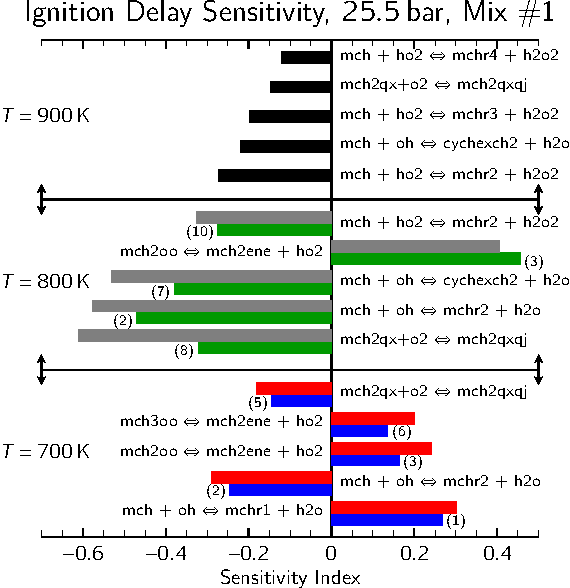
\includegraphics[width=10.5cm]{05-MCH/mch-sens}}
            {\caption{Sensitivity of the ignition delay to various reaction rates
                for Mix \#1 ($\phi=\num{1.0}$), \SI{25.5}{\bar} and three temperatures
                (\SIlist{700;800;900}{\kelvin}). At \SI{700}{\kelvin}, the sensitivity of the overall
                ignition delay is in red and the sensitivity of the first stage
                ignition delay is in blue. At \SI{800}{\kelvin}, the sensitivity of the overall
                ignition delay is in grey and the sensitivity of the first stage
                ignition delay is in green. At \SI{900}{\kelvin}, the sensitivity of the overall
                ignition delay is in black. Numbers in parentheses represent the
                ranking of the first stage sensitivity indices.}
            \label{fig:mch-sens}}
        \ffigbox[\FBwidth][\FBheight]
            {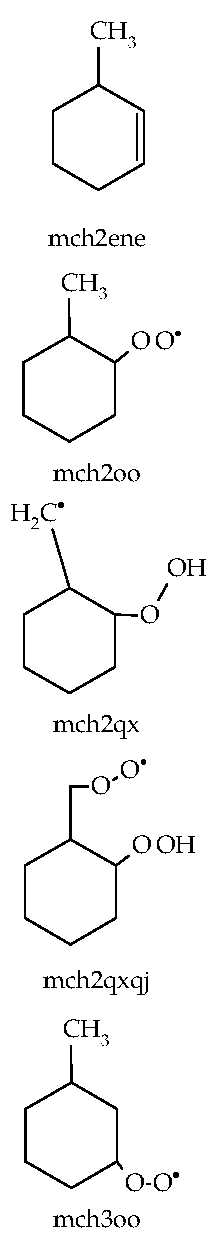
\includegraphics[height=18cm]{05-MCH/mch-species}}
            {\caption{Species mentioned in \cref{fig:mch-sens} or
                \cref{tab:mch-sens} and not included in \cref{fig:mch-path}.}
            \label{fig:mch-species}}
    \end{floatrow}
\end{figure}

In general, \cref{fig:mch-sens} shows that the ignition delay
is sensitive to different sets of reactions at the three
temperatures, although there is some overlap. The overlapping
reactions confound simple recommendations for rate improvements.
For instance, at \SI{700}{\kelvin}, increasing the overall ignition
delay will improve agreement with the experimental data, but at
\SI{800}{\kelvin}, the agreement is already quite good. Therefore,
adjusting any of the rates to improve the agreement with the overall
ignition delay at \SI{700}{\kelvin} will probably make the agreement
worse at \SI{800}{\kelvin}. However, the first stage ignition delays
at \SI{700}{\kelvin} and \SI{800}{\kelvin} are both under-predicted;
furthermore, two-stage ignition is predicted at temperatures for
which the experimental ignition is single stage. It should therefore
be possible to adjust several rate constants simultaneously to improve
agreement with the first stage ignition delay and not deteriorate
agreement with the overall ignition delay. To accomplish the
simultaneous improvement of agreement of first stage and overall
ignition delays, the rate constants of reactions that control the
second stage ignition delay may also need to be adjusted (where
second stage ignition delay is the difference between the overall
ignition delay and the first stage ignition delay).

Interestingly, the formation and destruction reactions of ROOH species
do not appear in \cref{fig:mch-sens}, despite their importance in
the destruction of ROO radicals, particularly at \SI{700}{\kelvin}
(see \cref{fig:mch-path}). This may be due to the fact that
formation of ROOH by reaction with HO$_2$ followed by consumption of ROOH
is a chain propagation path through the reactions ROO+HO$_2$=ROOH+O$_2$;
ROOH=RO+OH. In this sequence two radicals are formed (RO, OH) and two
radicals are consumed (ROO, HO$_2$). Thus, the formation of ROOH by
reaction with HO$_2$ and its subsequent destruction has a somewhat
neutral effect on the radical pool.

At \SI{900}{\kelvin}, the overall ignition delay is particularly sensitive
to reactions that form hydrogen peroxide, which decomposes to two
hydroxyl radicals as the temperature increases during the induction
period. Therefore, increasing the rate of formation of hydrogen peroxide
will increase the formation of hydroxyl radical and decrease the overall
ignition delay. At \SI{900}{\kelvin}, the overall ignition delay is
over-predicted, so to improve the results, the overall ignition delay
should be reduced (i.e. increasing the rates of reactions with negative
sensitivity will improve the comparison). In addition, many of the
reactions that are important at \SI{900}{\kelvin} are not important at
\SIlist{700;800}{\kelvin}, implying that changes made to the rates to
improve the high-temperature agreement will not significantly change the
agreement at lower temperature. In particular, the MCH+HO$_2$ rate constants
have not been measured or calculated to our knowledge and are based
on acyclic alkane rate constants \cite{Aguilera-Iparraguirre2008}. They have uncertainties of at
least a factor of 2 and as much as a factor of 10 based on the work
of \textcite{Aguilera-Iparraguirre2008}. Increasing these rate constants
would improve the agreement with the experimental ignition data at
\SI{900}{\kelvin} in the RCM and shock tube. Experimental measurements
and theoretical calculations are needed for the fuel+HO$_2$ reaction class to
reduce this uncertainty in the rate constants.

\section{Conclusions}

In this study, new experimental data are collected for methylcyclohexane
autoignition in a heated RCM. Following the work
of \textcite{Mittal2009}, three mixtures of MCH/O$_2$/ N$_2$/Ar at equivalence
ratios of $\phi=\numlist{0.5;1.0;1.5}$ are used and the ignition delays
are measured at compressed pressure of \SI{50}{\bar}, for compressed
temperatures in the range of \SIrange{690}{900}{\kelvin}. Two-stage
ignition phenomena are reported for the stoichiometric and rich
mixtures. However, substantial reactivity during the compression
stroke limited the temperature range over which ignition delays could
be reported, especially for the lean case. For these mixtures where the
fuel concentration was kept constant, the order of reactivity, in terms
of inverse overall ignition delay, is $\phi=\num{0.5}>\phi=\num{1.0}>\phi=\num{1.5}$.

In addition, an existing model for the combustion of MCH developed by
\textcite{Pitz2007} is updated with new reaction rates and pathways.
The new model shows good agreement with the overall ignition delays
measured in this study, as well as the overall ignition delays measured
in the studies of \textcite{Mittal2009,Vasu2009,Vanderover2009}. However,
the first stage ignition delays are uniformly under-predicted and in
several cases, first stage ignition is predicted by the model where
experimental ignition response shows no two-stage character. To help
understand the fuel decomposition pathways and the reactions controlling
the ignition, further analysis of the present mechanism is conducted.

First, reaction path analysis is conducted for low-, intermediate-, and
high-temperature ignition considered in this study. The results show that
MCH primarily decomposes by H-abstraction reactions involving OH and HO$_2$
radicals, followed by oxygen addition reactions. At low temperatures,
the oxygen addition is followed by isomerization to QOOH species and
second oxygen addition, leading to the low-temperature chain branching
characteristic of two-stage ignition. At intermediate temperatures, the
elimination of methylcyclohexene and HO$_2$ becomes competitive with the
isomerization reaction, leading to the NTC region of the overall ignition
delay. Finally, at high temperatures, MCH+HO$_2$ reactions form H$_2$O$_2$ and end
the NTC region.

Second, a brute force sensitivity analysis is conducted to identify the
reactions of the fuel and primary fuel radicals that control the ignition
process. The overall and first stage ignition events at low and intermediate
temperatures are primarily controlled by the initial reactions to form
fuel radicals, especially H-abstraction by OH. At high temperatures, the
controlling reactions are still the fuel radical formation reactions, but
now the ignition process is controlled by H-abstraction by hydroperoxyl
instead of hydroxyl. Combined, these analyses suggest that further
investigation of several of the low-temperature fuel decomposition
pathways is required and more accurate rate constants for fuel+HO$_2$
reactions are needed.

\end{document}
